
\section{mclique.rb 極大クリークの列挙\label{sect:mclique}}

本コマンドは、一般グラフから極大クリークを列挙する。
内部では\cite{UnoWeb}の\verb|mace|コマンドを利用している。

$G=(V,E)$を節点集合$V$と枝集合$E$を持つ無向グラフとすると、
$V$の部分集合の任意の節点に枝があるような$G$の誘導部分グラフをクリークと呼ぶ。
%$V$の部分集合$V'$に対して$V'$によって誘導される部分グラフ$G'=(V',E(V'))(E'=\{(u,v) \in E|u,v \in V'\}$が完全グラフとなっている$G$の誘導部分グラフをクリークとい>う。
また、あるクリークが他のクリークの真部分集合でなければ、それは極大クリークと呼ばれる(図\ref{fig:clique})。

\begin{figure}[htbp]
\begin{center}
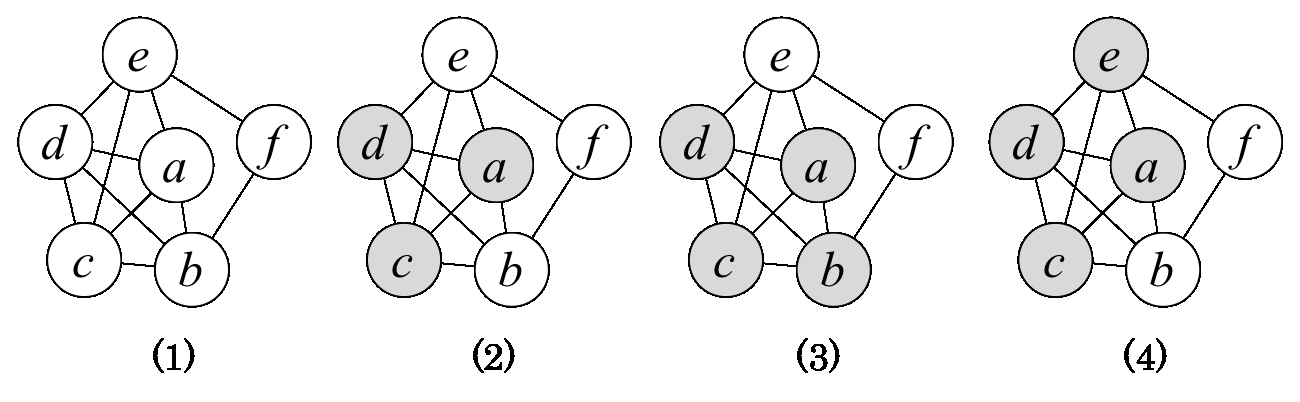
\includegraphics[scale=0.5]{./clique.eps}
\caption{一般グラフ(1)について、網掛けで示された部分グラフ(2)はクリークではあるが、
(3)や(4)に示されたクリークの真部分集合なので極大クリークではない。
一方で(3)や(4)はその他のどのクリークの真部分集合にはならないので極大である。
(3)と(4)は4つの頂点より構成されるが、そのうち3点が互いに共通している。
\label{fig:clique}}
\end{center}
\end{figure} 

一般的なケースにおいて、極大クリークを列挙するとその数が膨大になることが多い。
図\ref{fig:clique}の(3)と(4)のように、節点が重複するような極大クリークが多数存在するためである。
この問題を克服するアプローチがこれまでに幾つか提案されてきた。
ひとつは、完全グラフでなくても、ある程度の密度であれば完全グラフと見なしてしまおうというもので、
そのようなクリークは擬似クリークと呼ばれる。
しかしながら、時に擬似クリークは極大クリーク以上に列挙されるケースもあり、根本的な解決にならない。
他の方法としては、極大クリークを列挙した後で、似たクリークを併合していこうというアプローチであり、
世に存在する多くのクラスタリングのアルゴリズムが利用できる。
これは有望なアプローチではあるものの、列挙された極大クリークの数によっては実行時間が問題となる。
そこで、第三のアプローチとして、列挙対象である一般グラフを事前にクリーニングする(このようなクリーニングを「データ研磨」と呼ぶ)
ことで、そもそも列挙される極大クリークの数を大幅に減らしてしまおうという方法がある。
この方法は宇野らによって最近提案された方法で\cite{Uno2014}、データ研磨の数理的性質がより明らかになってくれば、
クリーク列挙において有効な方法論となっていくであろう。
第\ref{sect:mpolishing}節に示された\verb|mpolishing.rb|コマンドは、この手法を実装したものであり、
本コマンドと組み合わせて利用することで、グラフの本質をさほど変更することなく極大クリークの列挙数を劇的に少なくすることができる。

さて、本コマンドの入力データである一般グラフは、表\ref{tbl:cl_input}に示されるような、
枝データを節点ペアとして表したCSV形式で与える(図\ref{fig:clique} (1)に対応)。
グラフは無向グラフとして扱われ、島が複数あってもよい。

このグラフデータで極大クリークを列挙すると表\ref{tbl:cl_output}に示されるような形式で
クリークが列挙される。
\verb|id|項目がクリークのIDで、この項目が同じ行で一つのクリークが識別される。
\verb|id|=2のクリークが図\ref{fig:clique}(4)に対応し、
\verb|id|=3のクリークが図\ref{fig:clique}(3)に対応している。
その他にも、2つの節点から構成される極大クリーク$\{e,f\}$と$\{b,f\}$も列挙されている。
最後の\verb|size|項目は、極大クリークを構成する節点数である。

%さらに、\verb|no=,ne=|のパラメータを指定することで、列挙されたクリークについて、一つの極大クリークを節点としたグラフ
%(このような節点をクリーク節点、そしてグラフをクリーク節点グラフと呼ぶ)
%を出力することもできる。
%2つのクリークについて、共有される節点がある場合、それらのクリーク節点間に枝が張られる。
%表\ref{tbl:cl_output}に示された極大クリークに基づいて描画されクリーク節点グラフを
%図\ref{fig:cl_clnodeg}に、そして出力されるCSVデータを表\ref{tbl:cl_node},\ref{tbl:cl_edge}に示す。

\begin{table}[htbp]
\begin{center}
\begin{tabular}{cc}

\begin{minipage}{0.5\hsize}
\begin{center}
\caption{入力データ(枝データ)\label{tbl:cl_input}}
{\small
\begin{tabular}{cc}
\hline
node1&node2 \\
\hline
a&b \\
a&c \\
a&d \\
a&e \\
b&c \\
b&d \\
b&f \\
c&d \\
c&e \\
d&e \\
e&f \\
\hline
\end{tabular} 
}
\end{center}
\end{minipage}

\begin{minipage}{0.5\hsize}
\begin{center}
\caption{出力結果\label{tbl:cl_output}}
{\small
\begin{tabular}{cccc}
\hline
id&node1&node2&size\\
\hline
0&e&f&2\\
1&b&f&2\\
2&a&c&4\\
2&a&d&4\\
2&a&e&4\\
2&c&d&4\\
2&c&e&4\\
2&d&e&4\\
3&a&b&4\\
3&a&c&4\\
3&a&d&4\\
3&b&c&4\\
3&b&d&4\\
3&c&d&4\\
\hline
\end{tabular} 
}
\end{center}
\end{minipage}


\end{tabular} 
\end{center}
\end{table} 


%\begin{figure}[htbp]
%\begin{center}
%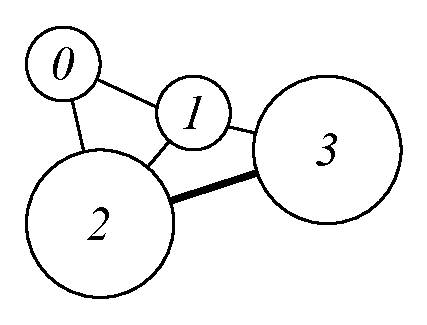
\includegraphics[scale=0.5]{./clnodeg.eps}
%\caption{クリーク節点グラフ。表\ref{tbl:cl_output}に示された4つの極大クリークを、それぞれ節点としたグラフ。
%節点内の数字はクリークIDを表し、節点の大きさはクリークを構成する節点数に比例して描画している。
%例えば、クリーク節点"2"は、$a,c,d,e$の4つの節点から構成され、"0"は$e,f$の2つの節点から構成されている。
%枝は、クリーク間に共通する節点数が1以上の場合に張られており、その太さはその数に比例して描画している。
%例えば、クリーク節点"2"と"0"の共通節点は1つの節点$e$のみである。
%クリーク節点"0"と"3"には共通節点がないので枝は張られない。
%\label{fig:cl_clnodeg}}
%\end{center}
%\end{figure} 


%\begin{table}[htbp]
%\begin{center}
%\begin{tabular}{cc}

%\begin{minipage}{0.5\hsize}
%\begin{center}
%\caption{クリーク節点グラフにおける節点データ\label{tbl:cl_node}}
%{\small
%\begin{tabular}{cc}
%\hline
%node&size \\
%\hline
%0&2 \\
%1&2 \\
%2&4 \\
%3&4 \\
%\hline
%\end{tabular} 
%}
%\end{center}
%\end{minipage}

%\begin{minipage}{0.5\hsize}
%\begin{center}
%\caption{クリーク節点グラフにおける枝データ\label{tbl:cl_edge}}
%{\small
%\begin{tabular}{ccc}
%\hline
%node1&node2&common \\
%\hline
%0&1&1 \\
%0&2&1 \\
%1&3&1 \\
%2&3&3 \\
%\hline
%\end{tabular} 
%}
%\end{center}
%\end{minipage}

%\end{tabular} 
%\end{center}
%\end{table} 



\subsection{書式}
\begin{verbatim}
書式) mclique.rb ei= ef= [ni=] [nf=] [o=] [l=] [u=] [-all] [-node] [-all] [-int] [log=] [T=] [--help]

  ファイル名指定
  ei=    : 枝データファイル
  ef=    : 枝データ上の2つの節点項目名(-intを指定した場合は指定できない)
  ni=    : 節点データファイル
  nf=    : 節点データ上の節点項目名(省略時は"node")
  o=     : 出力ファイル(クリークID-枝:-nodeを指定することでクリークID-節点に変更可能)
  l=     : クリークを構成する最小節点数(ここで指定したサイズより小さいクリークは列挙されない)
  u=     : クリークを構成する最大節点数(ここで指定したサイズより大きいクリークは列挙されない)
  -node  : 出力形式をクリークID-node名のペアとする。
  -all   : 極大クリークだけでなく、全クリークを列挙する。
  -int   : アイテムを整数とみなして処理する。
  log=   : パラメータの設定値をkey-value形式のCSVで保存するファイル名

  その他
  T= : ワークディレクトリ(default:/tmp)
  --help : ヘルプの表示
\end{verbatim}

\subsection{利用例}
\subsubsection*{Example 1: Basic Example}

Example illustrated from the above section.


\begin{Verbatim}[baselinestretch=0.7,frame=single]
$ more dat1.csv
node1,node2
a,b
a,c
a,d
a,e
b,c
b,d
b,f
c,d
c,e
d,e
e,f
$ mclique.rb i=dat1.csv f=node1,node2 o=result1.csv log=log1.csv
/Users/stephane/.rvm/gems/ruby-1.9.3-p448/gems/nysol-1.5-x86_64-darwin/lib/nysol/margs.rb:
154:in `block in initialize': I don't know such a argument: `i=' (RuntimeError)
	from /Users/stephane/.rvm/gems/ruby-1.9.3-p448/gems/nysol-1.5-x86_64-darwin/lib/nysol/mar
gs.rb:152:in `each'
	from /Users/stephane/.rvm/gems/ruby-1.9.3-p448/gems/nysol-1.5-x86_64-darwin/lib/nysol/mar
gs.rb:152:in `initialize'
	from /Users/stephane/.rvm/gems/ruby-1.9.3-p448/gems/nysol-1.5-x86_64-darwin/bin/mclique.r
b:124:in `new'
	from /Users/stephane/.rvm/gems/ruby-1.9.3-p448/gems/nysol-1.5-x86_64-darwin/bin/mclique.r
b:124:in `<top (required)>'
	from /Users/stephane/.rvm/rubies/ruby-1.9.3-p448/bin/mclique.rb:23:in `load'
	from /Users/stephane/.rvm/rubies/ruby-1.9.3-p448/bin/mclique.rb:23:in `<main>'
$ more result1.csv
result1.csv: No such file or directory
$ more cn1.csv
cn1.csv: No such file or directory
$ more ce1.csv
ce1.csv: No such file or directory
$ more log1.csv
log1.csv: No such file or directory
\end{Verbatim}
\subsubsection*{Example 2: Enumerate maximal cliques with size 4 or above}



\begin{Verbatim}[baselinestretch=0.7,frame=single]
$ mclique.rb i=dat1.csv f=node1,node2 l=4 o=result2.csv
/Users/stephane/.rvm/gems/ruby-1.9.3-p448/gems/nysol-1.5-x86_64-darwin/lib/nysol/margs.rb:
154:in `block in initialize': I don't know such a argument: `i=' (RuntimeError)
	from /Users/stephane/.rvm/gems/ruby-1.9.3-p448/gems/nysol-1.5-x86_64-darwin/lib/nysol/mar
gs.rb:152:in `each'
	from /Users/stephane/.rvm/gems/ruby-1.9.3-p448/gems/nysol-1.5-x86_64-darwin/lib/nysol/mar
gs.rb:152:in `initialize'
	from /Users/stephane/.rvm/gems/ruby-1.9.3-p448/gems/nysol-1.5-x86_64-darwin/bin/mclique.r
b:124:in `new'
	from /Users/stephane/.rvm/gems/ruby-1.9.3-p448/gems/nysol-1.5-x86_64-darwin/bin/mclique.r
b:124:in `<top (required)>'
	from /Users/stephane/.rvm/rubies/ruby-1.9.3-p448/bin/mclique.rb:23:in `load'
	from /Users/stephane/.rvm/rubies/ruby-1.9.3-p448/bin/mclique.rb:23:in `<main>'
$ more result2.csv
result2.csv: No such file or directory
\end{Verbatim}
\subsubsection*{Example 3: Enumerate all cliques with size of 3}



\begin{Verbatim}[baselinestretch=0.7,frame=single]
$ mclique.rb i=dat1.csv f=node1,node2 l=3 u=3 -all o=result3.csv
/Users/stephane/.rvm/gems/ruby-1.9.3-p448/gems/nysol-1.5-x86_64-darwin/lib/nysol/margs.rb:
154:in `block in initialize': I don't know such a argument: `i=' (RuntimeError)
	from /Users/stephane/.rvm/gems/ruby-1.9.3-p448/gems/nysol-1.5-x86_64-darwin/lib/nysol/mar
gs.rb:152:in `each'
	from /Users/stephane/.rvm/gems/ruby-1.9.3-p448/gems/nysol-1.5-x86_64-darwin/lib/nysol/mar
gs.rb:152:in `initialize'
	from /Users/stephane/.rvm/gems/ruby-1.9.3-p448/gems/nysol-1.5-x86_64-darwin/bin/mclique.r
b:124:in `new'
	from /Users/stephane/.rvm/gems/ruby-1.9.3-p448/gems/nysol-1.5-x86_64-darwin/bin/mclique.r
b:124:in `<top (required)>'
	from /Users/stephane/.rvm/rubies/ruby-1.9.3-p448/bin/mclique.rb:23:in `load'
	from /Users/stephane/.rvm/rubies/ruby-1.9.3-p448/bin/mclique.rb:23:in `<main>'
$ more result3.csv
result3.csv: No such file or directory
\end{Verbatim}



